\chapter{Realization}
\minitoc
\newpage

\setcounter{secnumdepth}{0} % Set the section counter to 0 so next section is not counted in toc
% ----------------------- Introduction ----------------------- %
\section{Introduction}
This chapter details the implementation and deployment of Navoy's modernized AI travel platform, focusing on the practical network infrastructure and microservices deployment approach. I present the technical realization of the network architecture, DevSecOps pipeline implementation, and the solutions that enable scalability and reliability.

The implementation encompasses Azure services for development support and shared resources, AWS services for production deployment, microservices containerization, and comprehensive monitoring with observability tools. This approach prioritizes practical deployment capabilities while maintaining the platform's core functionality and performance requirements.

\setcounter{secnumdepth}{2} % Resume counting the sections for the toc with a depth of 2 (Sections and sub-sections)
% ----------------------------------- SECTIONS (v) ----------------------------------- %
% ----------------------- Development Environment Setup ----------------------- %
\section{Development Environment Setup}
The modernization project required establishing a comprehensive development environment that supports microservices development, containerization, and DevSecOps practices.

\subsection{Local Development Environment}
I configured a containerized development environment using Docker Compose to ensure consistency across all development environments:

\begin{itemize}
    \item \textbf{Docker Desktop:} Installed for container management and local Kubernetes testing
    \item \textbf{VS Code with DevContainers:} Configured development containers for each microservice with language-specific tooling
    \item \textbf{Git Workflow:} Established GitFlow branching strategy with feature branches, develop, and main branches
    \item \textbf{Environment Variables:} Implemented secure environment variable management using .env files and Docker secrets
\end{itemize}

\subsection{Service-Specific Development Setup}

\subsubsection*{\underline{Envoy Proxy (REST Gateway)}}
\begin{itemize}
    \item \textbf{Service Mesh:} Envoy Proxy for advanced traffic management and load balancing
    \item \textbf{Configuration:} YAML-based configuration for routing, rate limiting, and caching
    \item \textbf{Redis Integration:} Redis for rate limiting and response caching
    \item \textbf{Authentication:} JWT token validation and authorization middleware
\end{itemize}

\subsubsection*{\underline{NestJS Services (User Service, Trip Generator, Travel Data Sync)}}
\begin{itemize}
    \item \textbf{Runtime:} Node.js 18 LTS with npm for package management
    \item \textbf{Framework:} NestJS for scalable server-side applications with TypeScript
    \item \textbf{Database Connectivity:} PostgreSQL and MongoDB client libraries with Prisma/Mongoose
    \item \textbf{Testing Setup:} Jest for unit testing with comprehensive decorator and service testing
    \item \textbf{Code Quality:} ESLint for code linting, Prettier for code formatting, Husky for Git hooks
\end{itemize}

\subsubsection*{\underline{Node.js Services (Vector Store Service)}}
\begin{itemize}
    \item \textbf{Runtime:} Node.js 18 LTS with npm for package management
    \item \textbf{gRPC Integration:} gRPC server implementation for high-performance communication
    \item \textbf{Database Connectivity:} ChromaDB client libraries for vector operations
    \item \textbf{Message Queue:} RabbitMQ consumer integration for embedding generation
    \item \textbf{Code Quality:} ESLint for code linting, Prettier for code formatting
\end{itemize}

% ----------------------- Cloud Infrastructure Setup ----------------------- %
\section{Cloud Infrastructure Setup}
The implementation of Navoy's AI travel platform follows a practical approach that leverages Azure for development support and shared resources, while AWS hosts the production infrastructure including the container registry, secrets management, and Kubernetes cluster.

\subsection{Azure Infrastructure for Development and Shared Resources}
Azure provides the foundation for development activities and shared infrastructure components, enabling efficient development workflows and resource sharing.

\begin{figure}[H]
    \centering
    \makebox[\textwidth]{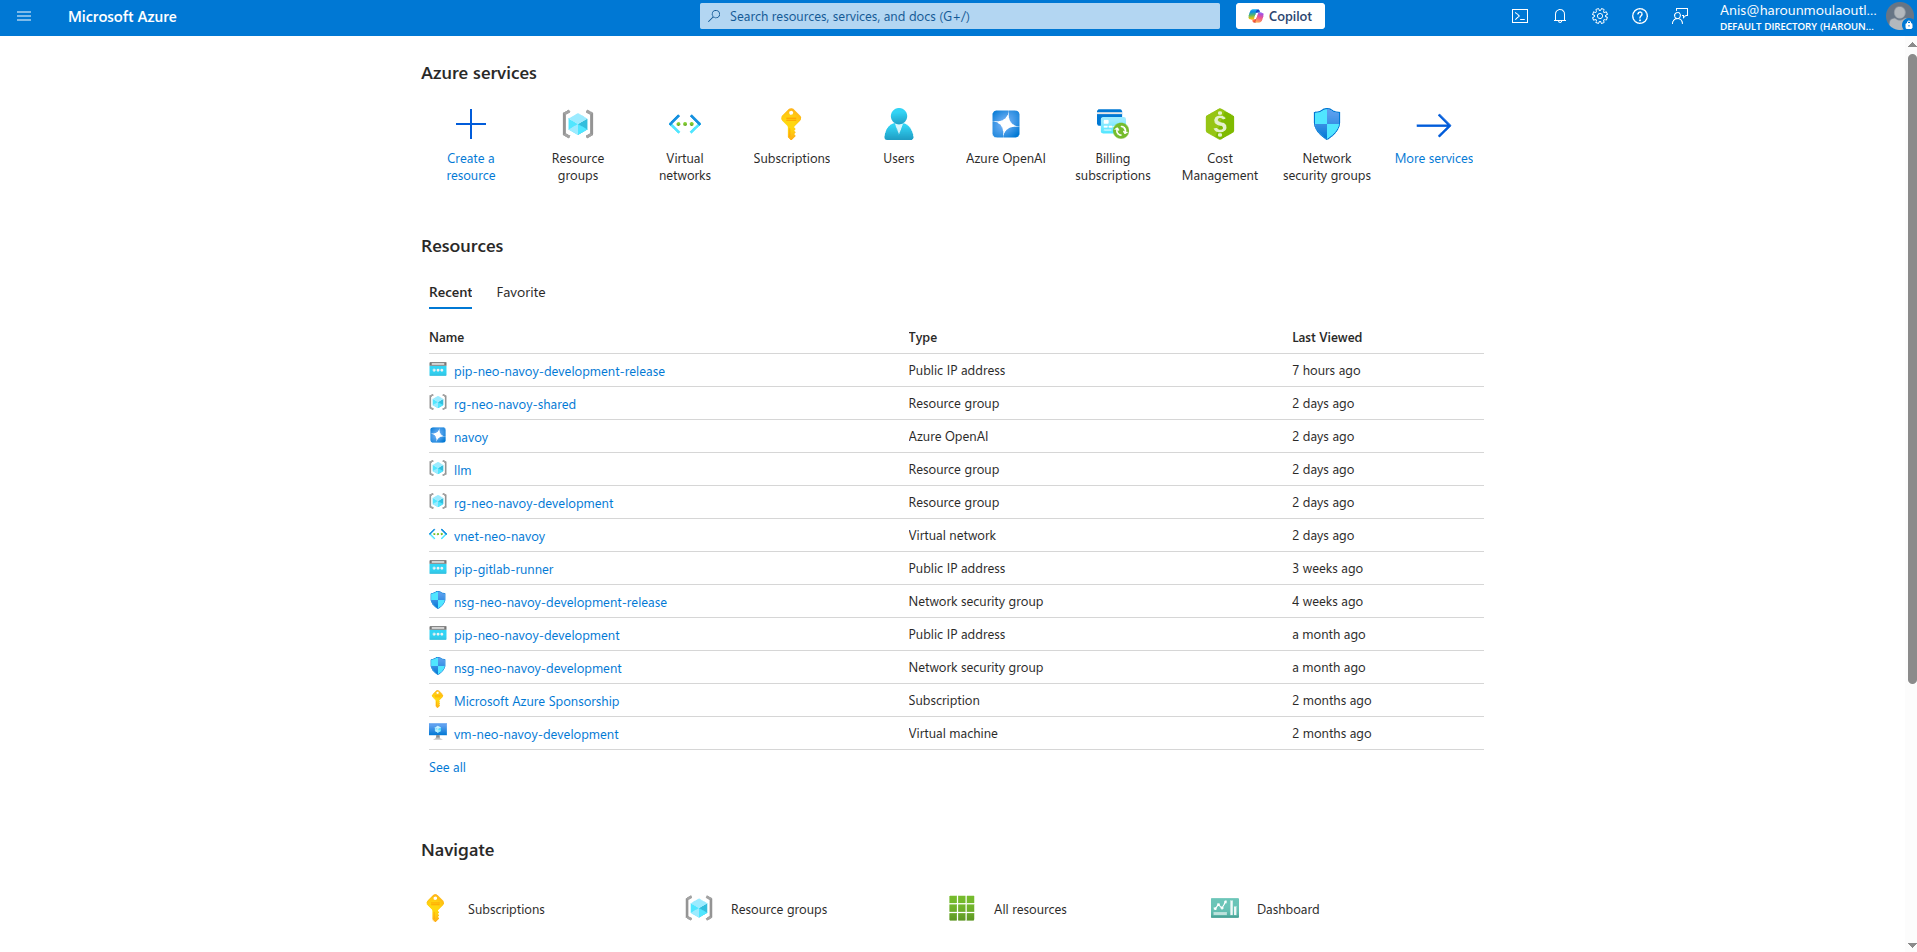
\includegraphics[width=\linewidth]{src/assets/images/azure-used-services.png}}
    \caption{Azure Services List Overview}
    \label{fig:azure-services-list}
\end{figure}

\subsubsection*{\underline{Development Resource Group Configuration}}
I configured Azure development resource groups to support the complete development lifecycle. The setup includes virtual machines for development environments, network security groups for controlled access, and Azure DevOps integration for continuous deployment validation. Each development environment mirrors the production setup to ensure deployment consistency and reduce environment-specific issues.

\subsubsection*{\underline{Azure OpenAI Service Integration}}
The platform leverages Azure OpenAI Service for AI model development and testing. I configured access to GPT models for trip generation prototyping, established proper API key management, and implemented usage monitoring to optimize costs during development. The service provides consistent AI capabilities for testing before production deployment.

\subsubsection*{\underline{Shared Resource Group Implementation}}
I implemented shared resource groups hosting GitLab runners and other common infrastructure components. The configuration includes custom GitLab runner instances for CI/CD pipeline execution, shared monitoring tools, and centralized logging infrastructure. This approach optimizes resource utilization and provides consistent tooling across development teams.

\begin{figure}[H]
    \centering
    \makebox[\textwidth]{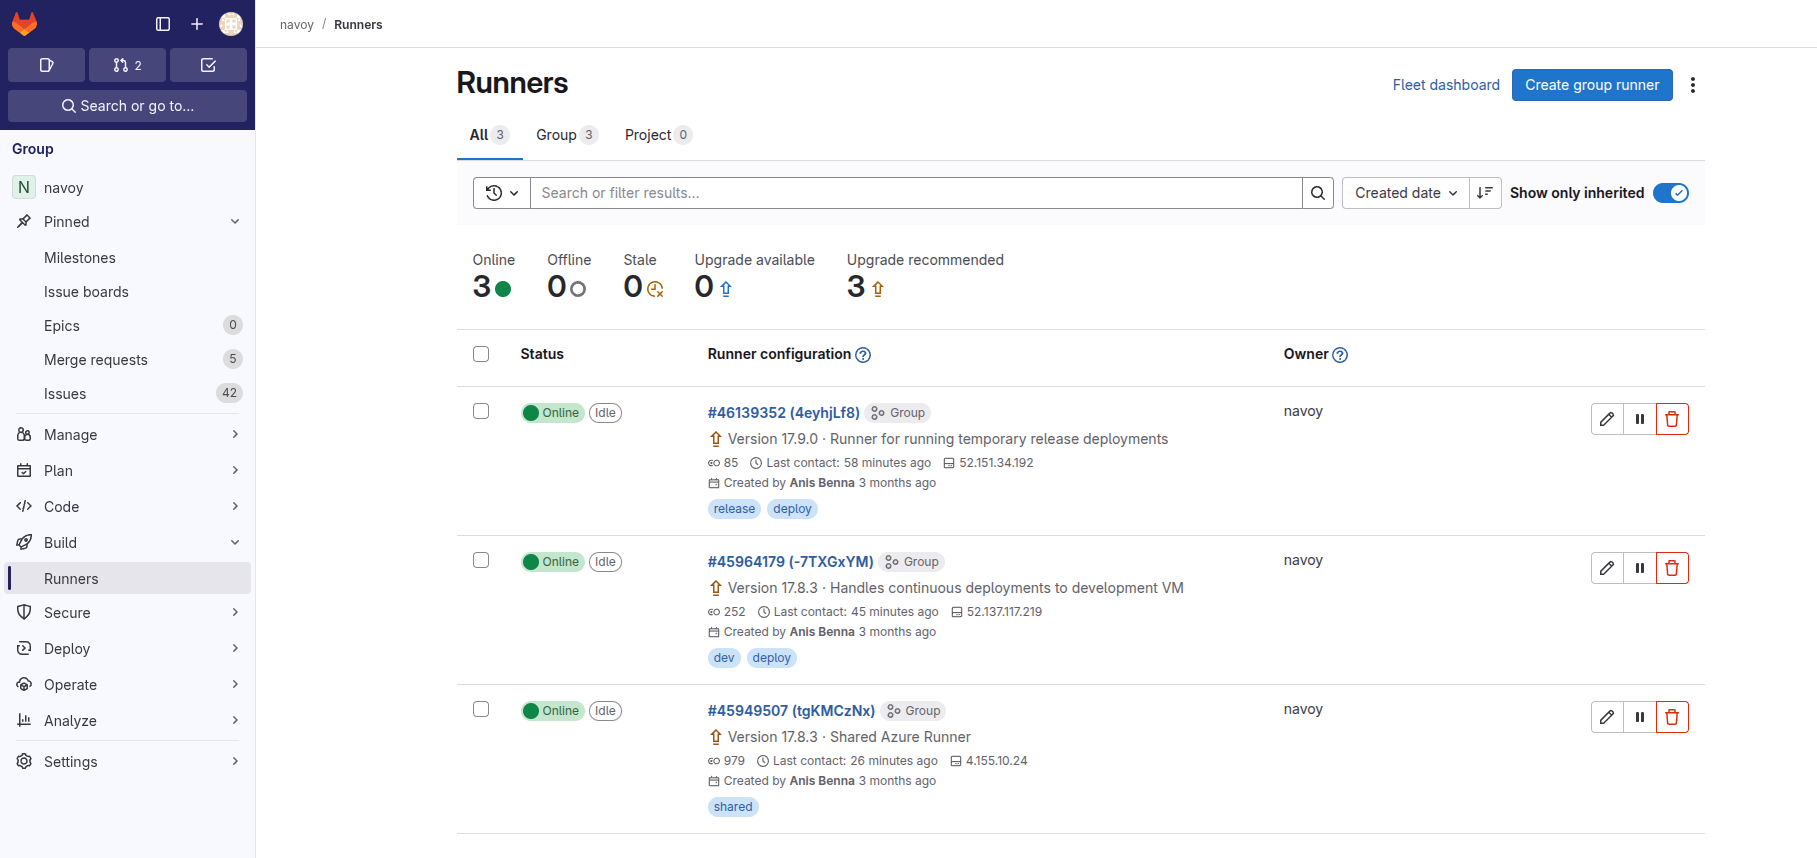
\includegraphics[width=\linewidth]{src/assets/images/gitlab-runners-list.png}}
    \caption{GitLab Runners Configuration for CI/CD Pipeline Execution}
    \label{fig:gitlab-runners-list}
\end{figure}

\subsection{AWS Production Infrastructure Implementation}
AWS serves as the primary production environment, hosting the core application components with comprehensive security and scalability features.

\subsubsection*{\underline{VPC Architecture for EKS Cluster}}
I implemented a dedicated VPC architecture designed specifically for the EKS cluster deployment. The configuration includes public subnets for load balancers and NAT gateways, private subnets for application workloads, and isolated subnets for databases. Each subnet tier includes appropriate route tables, security groups implementing least-privilege access, and VPC endpoints for secure access to AWS services without internet routing.

\subsubsection*{\underline{Container Registry and Secrets Management}}
AWS ECR serves as the centralized container registry for all Docker images built during CI runs. I configured repository policies for image lifecycle management, vulnerability scanning for security compliance, and cross-region replication for availability. AWS Secrets Manager handles all application secrets and Terraform state secrets with automatic rotation policies and fine-grained access controls.

\subsubsection*{\underline{EKS Cluster Configuration}}
The production EKS cluster implements industry best practices for security and scalability. I configured managed node groups with appropriate instance types, implemented cluster autoscaling for dynamic workload management, and established RBAC policies for service access control. The cluster includes network policies for pod-to-pod communication control and integration with AWS services through service accounts and IAM roles.

\subsubsection*{\underline{AWS Bedrock Integration}}
AWS Bedrock is integrated within the production environment to provide managed access to advanced foundation models, specifically Anthropic Claude models for enhanced AI capabilities. I configured secure API access through AWS IAM roles and policies, enabling the Trip Generator Service to leverage Bedrock's foundation models for trip evaluation, optimization, and advanced recommendation generation. The integration maintains data privacy and security while providing scalable access to state-of-the-art AI models without infrastructure management overhead.

\subsection{Load Balancing and Traffic Management}
The platform implements focused load balancing using AWS services to ensure reliable performance and security for production workloads.

\subsubsection*{\underline{Application Load Balancer Configuration}}
I deployed AWS Application Load Balancer as the single entry point for all external traffic. The configuration includes SSL/TLS termination using AWS Certificate Manager, path-based routing to the Kubernetes cluster, and integration with AWS WAF for application-layer protection. Health checks ensure automatic removal of unhealthy instances and seamless traffic routing.

\subsubsection*{\underline{Kubernetes Ingress Implementation}}
Within the EKS cluster, NGINX ingress controller handles internal service routing and traffic distribution. I configured ingress rules for each microservice, implemented SSL termination for internal traffic, and established rate limiting policies. The ingress controller integrates with the cluster autoscaler for dynamic scaling based on traffic patterns.

\subsubsection*{\underline{Auto-scaling Integration}}
The platform implements comprehensive auto-scaling using Kubernetes Horizontal Pod Autoscaler (HPA) and Vertical Pod Autoscaler (VPA). I configured CPU and memory-based scaling policies, custom metrics for application-specific scaling, and cluster-level scaling through AWS managed node groups. This ensures optimal resource utilization and cost management.

\begin{figure}[H]
    \centering
    \makebox[\textwidth]{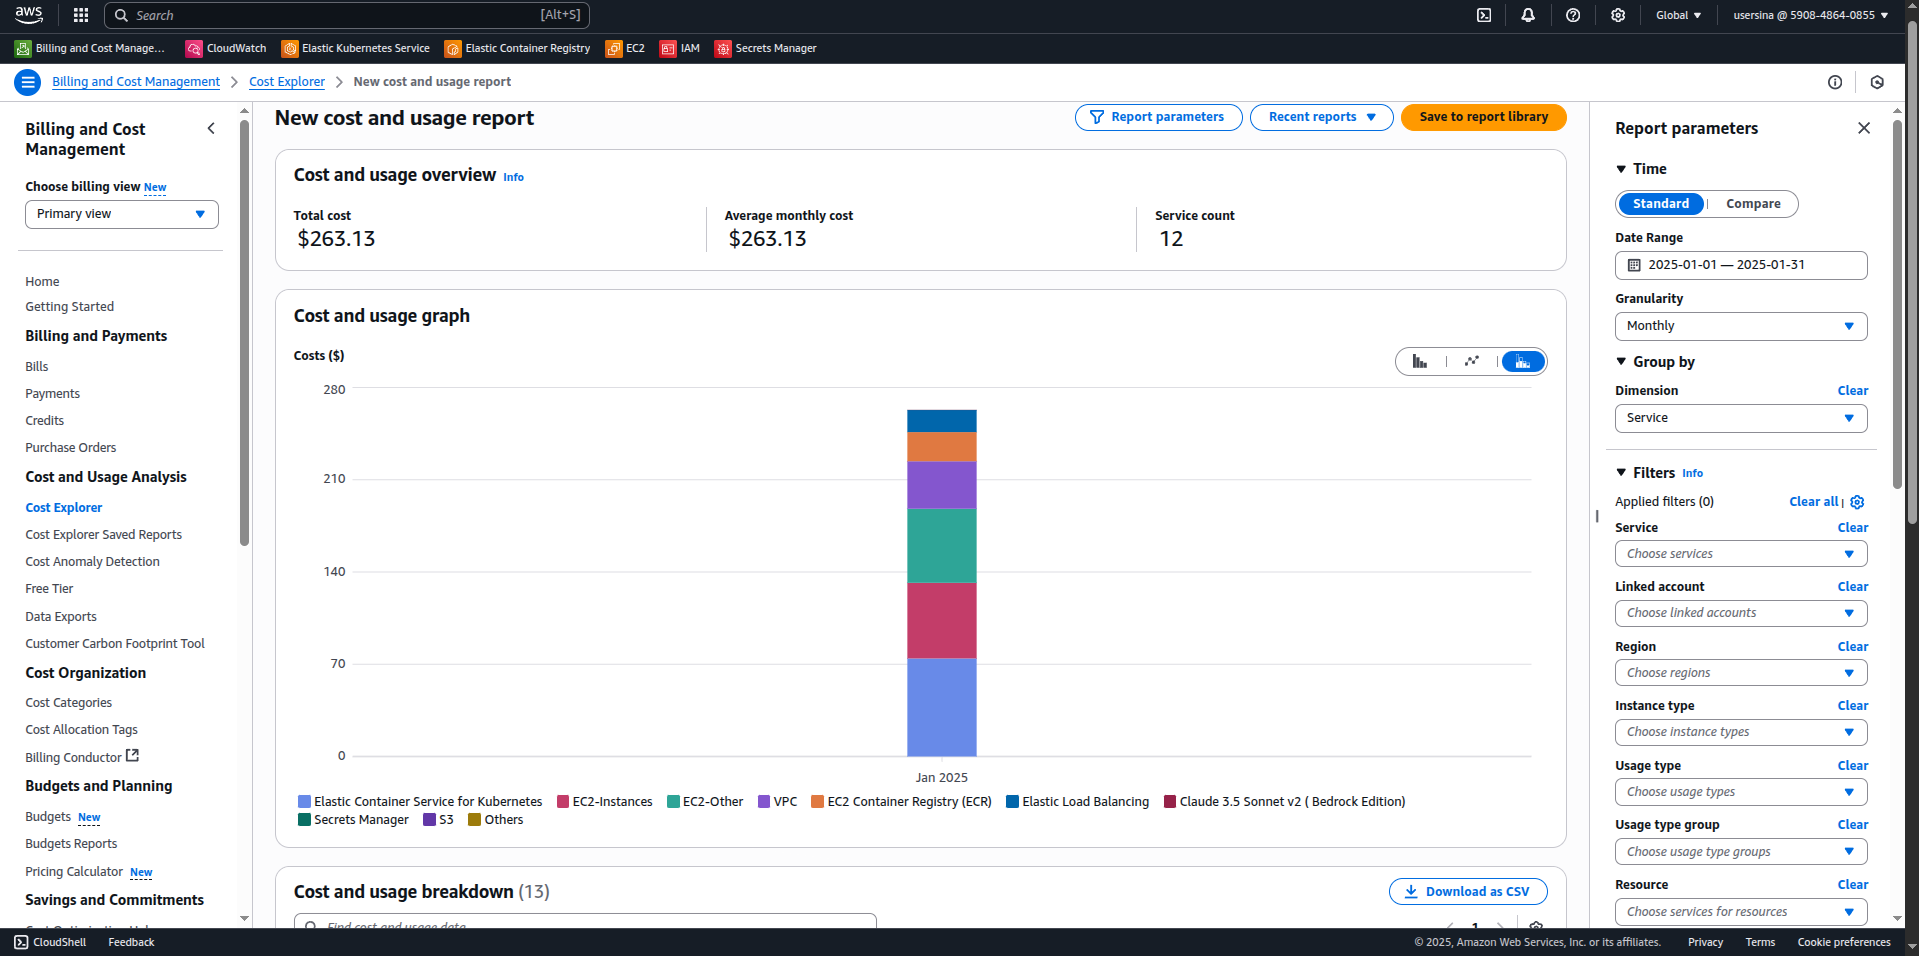
\includegraphics[width=\linewidth]{src/assets/images/aws-billing-monitoring.png}}
    \caption{AWS Cost Monitoring and Billing Dashboard Implementation}
    \label{fig:aws-billing-monitoring}
\end{figure}

% ----------------------- Network Security Implementation ----------------------- %
\section{Network Security Implementation}
Security is paramount for Navoy's AI travel platform, requiring comprehensive network security measures focused on the AWS production environment while maintaining secure development practices in Azure.

\subsection{Perimeter Security and DDoS Protection}
I implemented focused perimeter security to protect the platform from external threats and ensure service availability during attack scenarios.

\subsubsection*{\underline{Web Application Firewall Deployment}}
AWS WAF is deployed with custom rule sets tailored for travel industry applications. The configuration includes OWASP Top 10 protection, rate limiting rules based on user behavior patterns, geolocation filtering for compliance requirements, and custom rules for API endpoint protection. I created specific rule groups for protecting AI model endpoints, payment processing paths, and user authentication flows with the ALB integration.

\subsubsection*{\underline{DDoS Protection Configuration}}
I implemented AWS Shield Standard for basic DDoS protection across all AWS resources, with always-on traffic monitoring and automatic attack mitigation. The configuration includes custom thresholds based on normal traffic patterns and integration with CloudWatch for attack analytics. For the development environment, Azure DDoS Protection Standard provides similar protection for development resources.

\subsubsection*{\underline{API Gateway Security}}
Security at the REST gateway service level includes rate limiting with burst capacity, authentication token validation, request size limits, and IP allowlisting for administrative functions. I configured different rate limits for various user tiers and implemented progressive penalties for abusive behavior patterns within the Kubernetes deployment.

\subsection{Network Segmentation and Security Architecture}
The platform implements network segmentation with security best practices focused on the EKS cluster and supporting AWS infrastructure.

\subsubsection*{\underline{VPC Isolation and Segmentation}}
The EKS cluster operates within a dedicated VPC with private subnets for enhanced security. I implemented network segmentation using security groups and NACLs to restrict traffic to only necessary ports and protocols. Database resources are deployed in isolated subnets with dedicated security groups restricting access to authorized services only.

\subsubsection*{\underline{Kubernetes Network Policies}}
I deployed Kubernetes Network Policies for fine-grained control over pod-to-pod communication within the EKS cluster. The configuration includes service-specific policies, database access restrictions, and external API communication controls. Each microservice operates within its own network segment with explicit allow rules for required communications and namespace-based segmentation.

\subsubsection*{\underline{Service-to-Service Communication Security}}
Internal services communicate through private networking with security group rules enforcing least-privilege access. I implemented TLS encryption for service-to-service communication and configured service accounts with appropriate IAM roles for secure access to AWS services without requiring hardcoded credentials.

\subsection{Network Monitoring and Security Observability}
Comprehensive monitoring and security observability provide visibility into network traffic and enable rapid response to security incidents across the AWS infrastructure.

\subsubsection*{\underline{VPC Flow Logs and Analysis}}
I implemented comprehensive VPC Flow Logs collection within the EKS cluster VPC with integration into CloudWatch for automated analysis. The system detects anomalous traffic patterns, unauthorized access attempts, and potential security incidents. Flow logs are processed with alerting for suspicious activities and integration with security incident response procedures.

\subsubsection*{\underline{Security Hub Integration}}
AWS Security Hub provides centralized security findings and compliance status monitoring across all AWS resources. I configured automated security assessments, compliance reporting for industry standards, and integration with incident response workflows. The system aggregates security findings from multiple AWS security services for comprehensive visibility.

\subsubsection*{\underline{CloudTrail Logging and Monitoring}}
AWS CloudTrail provides comprehensive API call logging for security audit trails and compliance monitoring. I configured CloudTrail to capture all management events, data events for sensitive resources, and integration with CloudWatch for real-time alerting on suspicious API activities. This ensures complete audit trails for security investigations and compliance requirements.

% ----------------------- Microservices Implementation ----------------------- %
\section{Microservices Implementation}
This section details the technical implementation of each microservice according to the architecture defined in Chapter 3.

\begin{figure}[H]
    \centering
    \makebox[\textwidth]{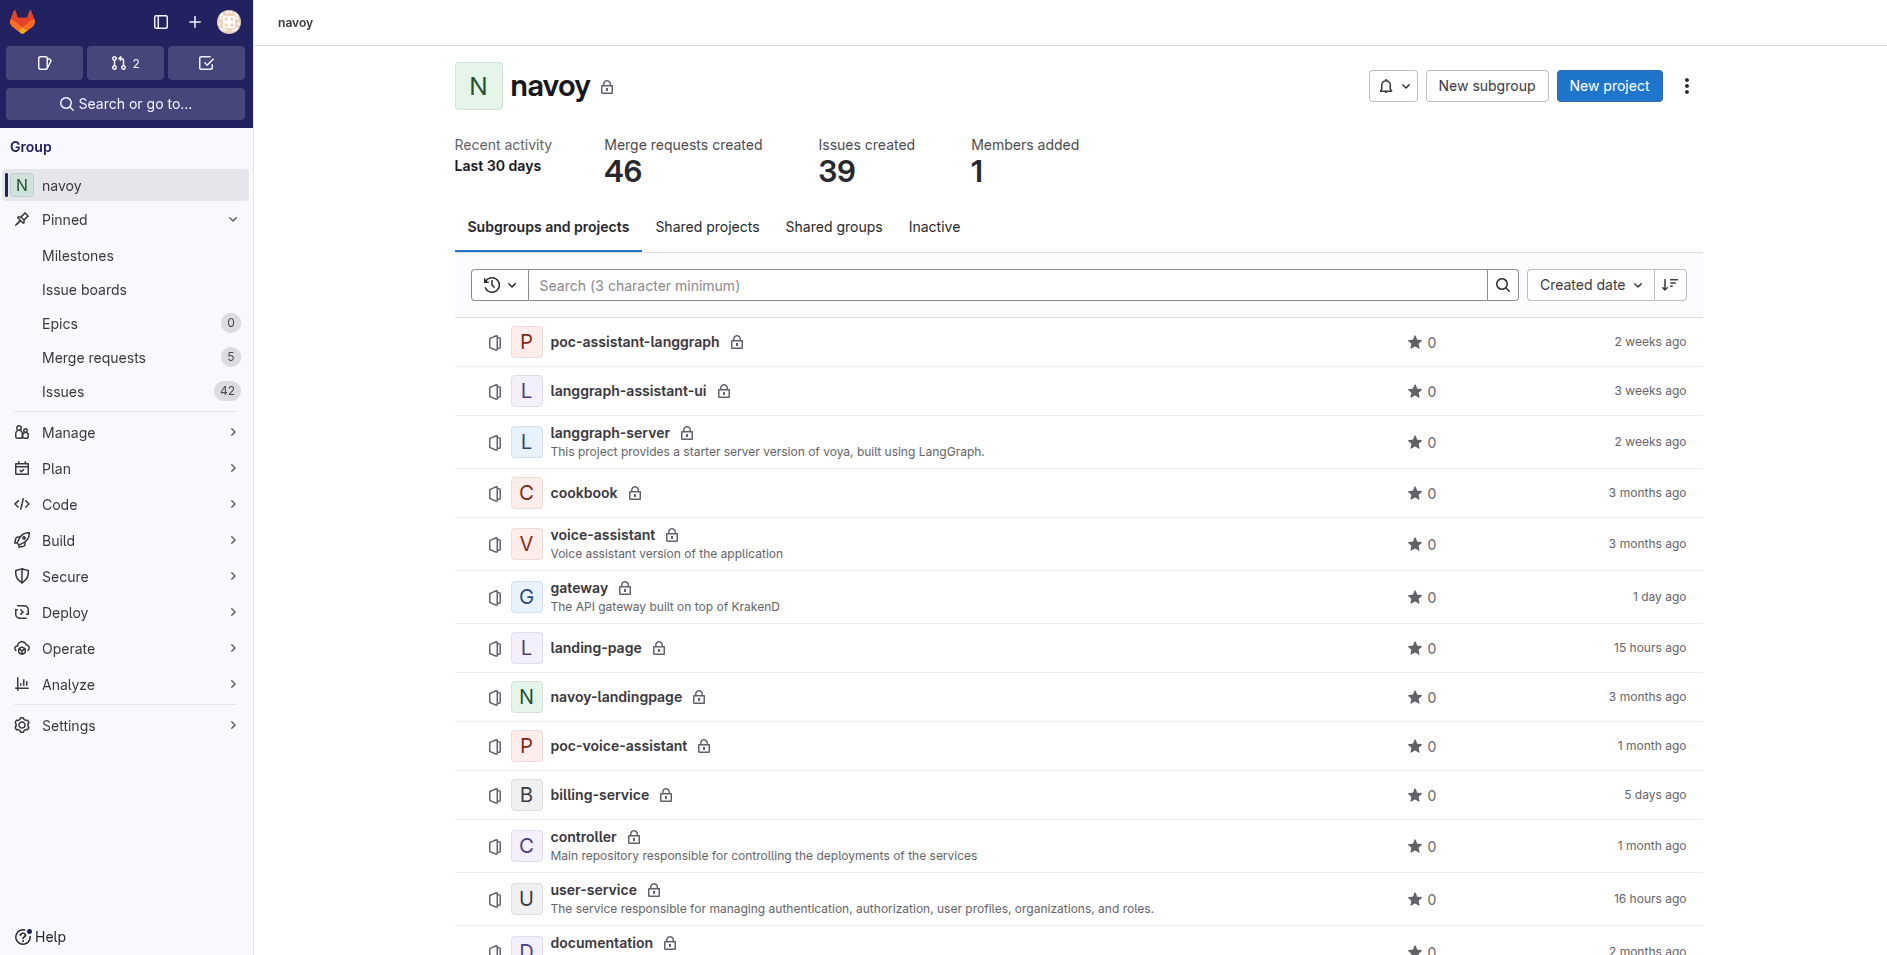
\includegraphics[width=\linewidth]{src/assets/images/gitlab-navoy-group.png}}
    \caption{GitLab Group Structure - Navoy Microservices Repositories Overview}
    \label{fig:gitlab-navoy-group}
\end{figure}

\subsection{REST Gateway Service Implementation}
The gateway service serves as the central entry point for all external requests and implements comprehensive API management capabilities using Envoy Proxy.

\subsubsection*{\underline{Core Features Implementation}}
\begin{itemize}
    \item \textbf{Envoy Proxy Configuration:} Configured Envoy as a service mesh proxy with advanced routing, load balancing, and traffic management
    \item \textbf{Redis Rate Limiting:} Implemented rate limiting using Envoy's rate limit service with Redis backend for distributed rate limiting
    \item \textbf{JWT Authentication Filter:} Configured Envoy JWT authentication filter for token validation and authorization
    \item \textbf{Dynamic Routing:} Implemented intelligent request routing to backend services with health checks and circuit breakers
    \item \textbf{OpenAPI Documentation:} Generated comprehensive API documentation with automatic service discovery
\end{itemize}

\subsubsection*{\underline{Performance Optimizations}}
\begin{itemize}
    \item Implemented response caching with Redis for frequently accessed endpoints
    \item Added request compression using gzip middleware
    \item Configured connection pooling for database and external API connections
    \item Implemented graceful shutdown handling for zero-downtime deployments
\end{itemize}

\subsection{User Service Implementation}
The user service manages authentication, authorization, and user profile management with multi-tenancy support.

\subsubsection*{\underline{Authentication System}}
\begin{itemize}
    \item \textbf{JWT Implementation:} Used jsonwebtoken library with RS256 algorithm for secure token generation
    \item \textbf{Password Security:} Implemented bcrypt hashing with salt rounds for password storage
    \item \textbf{Multi-Factor Authentication:} Integrated TOTP-based 2FA using speakeasy library
    \item \textbf{OAuth 2.0 Integration:} Configured Google and Microsoft OAuth providers using passport.js
\end{itemize}

\subsubsection*{\underline{Database Schema Design}}
\begin{itemize}
    \item Designed PostgreSQL schema with users, organizations, roles, and permissions tables
    \item Implemented row-level security for multi-tenant data isolation
    \item Added database migrations using Knex.js for schema versioning
    \item Configured connection pooling and read replicas for performance
\end{itemize}

\subsection{Trip Generator Service Implementation}
The trip generator service is the core AI-powered component that creates personalized travel itineraries.

\subsubsection*{\underline{AI Integration Architecture}}
The Trip Generator Service implements intelligent model selection and prompt engineering for optimal travel itinerary generation. I integrated LiteLLM as a unified proxy to access multiple AI models including OpenAI GPT-4 for creative trip planning and GPT-3.5-turbo for budget-conscious recommendations. Additionally, AWS Bedrock provides managed access to Anthropic Claude models within the production environment for trip evaluation and optimization tasks. The service implements asynchronous processing with proper error handling and response parsing to extract structured travel data from AI-generated content across all integrated model providers.

\subsubsection*{\underline{Asynchronous Processing}}
\begin{itemize}
    \item \textbf{AWS Lambda Integration:} Implemented serverless functions for handling trip generation requests asynchronously
    \item \textbf{Task Status Tracking:} Added Redis-based task status tracking for real-time progress updates
    \item \textbf{Error Handling:} Implemented retry mechanisms with exponential backoff for failed AI requests
    \item \textbf{Load Balancing:} Configured multiple Lambda function instances for horizontal scaling
\end{itemize}

\subsection{Data Synchronization Implementation}
The travel data sync service maintains fresh travel data from external APIs with scheduled updates and change detection.

\subsubsection*{\underline{External API Integration}}
\begin{itemize}
    \item \textbf{Viator API Adapter:} Implemented REST client with authentication and rate limiting
    \item \textbf{Amadeus Integration:} Added flight and hotel data synchronization with API key rotation
    \item \textbf{Data Transformation:} Created ETL pipelines for normalizing data from different providers
    \item \textbf{Change Detection:} Implemented checksum-based change detection to optimize sync operations
\end{itemize}

\subsubsection*{\underline{Scheduling and Performance}}
\begin{itemize}
    \item Configured AWS EventBridge for cron-based scheduled synchronization tasks
    \item Implemented batch processing for large datasets with progress tracking
    \item Added database indexing strategies for optimal query performance
    \item Created data archival processes for managing storage costs
\end{itemize}

\subsection{Vector Store Service Implementation}
The vector store service provides high-performance semantic search capabilities using ChromaDB and gRPC communication.

\subsubsection*{\underline{gRPC Server Implementation}}
\begin{itemize}
    \item \textbf{Protocol Buffer Definitions:} Defined comprehensive .proto files for vector operations and similarity queries
    \item \textbf{Node.js gRPC Server:} Implemented high-performance gRPC server using @grpc/grpc-js library
    \item \textbf{Streaming Support:} Added bi-directional streaming for batch vector operations and real-time similarity searches
    \item \textbf{Error Handling:} Implemented comprehensive error handling with proper gRPC status codes and metadata
\end{itemize}

\subsubsection*{\underline{ChromaDB Integration}}
\begin{itemize}
    \item \textbf{Vector Database Management:} Configured ChromaDB collections for travel content embeddings
    \item \textbf{Embedding Storage:} Implemented efficient storage and retrieval of travel destination and activity embeddings
    \item \textbf{Similarity Search:} Added optimized similarity search algorithms with configurable distance metrics
    \item \textbf{Index Management:} Implemented automated index optimization and maintenance procedures
\end{itemize}

\subsubsection*{\underline{RabbitMQ Consumer Integration}}
\begin{itemize}
    \item \textbf{Embedding Generation:} Implemented RabbitMQ consumers for processing embedding generation requests
    \item \textbf{Asynchronous Processing:} Added queue-based processing for large-scale embedding operations
    \item \textbf{Dead Letter Handling:} Configured dead letter queues for failed embedding generation attempts
    \item \textbf{Scalability:} Implemented horizontal scaling with multiple consumer instances
\end{itemize}

% ----------------------- Infrastructure and Deployment ----------------------- %
\section{Infrastructure and Deployment}
This section covers the infrastructure setup, containerization strategy, and deployment automation that enables the platform's scalability and reliability.

\subsection{Containerization Strategy}
Each microservice was containerized using Docker with optimized multi-stage builds to minimize image sizes and enhance security.

\subsubsection*{\underline{Docker Implementation}}
I implemented multi-stage Docker builds for all microservices to minimize image sizes and enhance security. Each service uses official Alpine Linux base images with non-root user configurations. The build process separates the dependency installation phase from the runtime phase, ensuring only necessary files are included in the final container image. This approach significantly reduces the attack surface and improves deployment speed.

\subsubsection*{\underline{Container Security Implementation}}
\begin{itemize}
    \item \textbf{Base Image Security:} Used official Alpine Linux images for minimal attack surface
    \item \textbf{Non-root Users:} Configured all containers to run with non-privileged users
    \item \textbf{Vulnerability Scanning:} Integrated Trivy scanner in CI/CD pipeline for image vulnerability assessment
    \item \textbf{Secrets Management:} Implemented external secret injection avoiding secrets in container images
\end{itemize}

\subsection{Kubernetes Deployment Architecture}
The platform is deployed on a self-managed Kubernetes cluster with comprehensive resource management and scaling capabilities.

\subsubsection*{\underline{Cluster Configuration}}
\begin{itemize}
    \item \textbf{EKS Setup:} Deployed managed Kubernetes cluster using Amazon EKS with managed node groups
    \item \textbf{Network Configuration:} Configured VPC CNI for pod networking with security groups for pods
    \item \textbf{Storage Configuration:} Implemented EBS CSI driver for persistent storage with automated backup
    \item \textbf{Load Balancing:} Deployed AWS Load Balancer Controller for ALB integration with Kubernetes ingress
\end{itemize}

\subsubsection*{\underline{Helm Charts Implementation}}
Created standardized Helm charts for consistent deployment across environments. Each microservice has its own chart with configurable values for different environments. The charts include deployment specifications, service configurations, ingress rules, and persistent volume claims. I implemented template-based configuration management allowing easy customization of resource limits, replica counts, and environment-specific settings while maintaining consistency across deployments.

\subsection{Infrastructure as Code Implementation}
Implemented Terraform for infrastructure provisioning and management with version control and state management.

\subsubsection*{\underline{Terraform Configuration}}
\begin{itemize}
    \item \textbf{AWS Provider Setup:} Configured AWS provider with role-based access and resource tagging
    \item \textbf{VPC and Networking:} Created isolated VPCs with public/private subnets and NAT gateways
    \item \textbf{EKS Cluster:} Provisioned managed Kubernetes cluster with worker node auto-scaling
    \item \textbf{RDS Databases:} Set up managed PostgreSQL instances with Multi-AZ deployment
    \item \textbf{ElastiCache:} Configured Redis clusters for caching and session management
\end{itemize}

\subsubsection*{\underline{Environment Management}}
\begin{itemize}
    \item Created separate Terraform workspaces for staging and production environments
    \item Implemented Terraform state locking using S3 backend with DynamoDB
    \item Added automated infrastructure drift detection and remediation
    \item Configured resource lifecycle management and cost optimization
\end{itemize}

% ----------------------- DevSecOps Pipeline Implementation ----------------------- %
\section{DevSecOps Pipeline Implementation}
The CI/CD pipeline integrates security at every stage while maintaining rapid deployment capabilities and comprehensive testing.

\subsection{GitLab CI/CD Pipeline Architecture}
Implemented a comprehensive GitLab CI/CD pipeline with security scanning, automated testing, and deployment automation.

\subsubsection*{\underline{Pipeline Stages}}
The GitLab CI/CD pipeline consists of five main stages: testing, security scanning, building, staging deployment, and production deployment. Each stage includes specific jobs for unit testing, code coverage analysis, static security analysis, container security scanning, image building, and automated deployment. The pipeline uses Docker BuildKit for optimized container builds and includes comprehensive artifact collection for test results and security reports.

\begin{figure}[H]
    \centering
    \makebox[\textwidth]{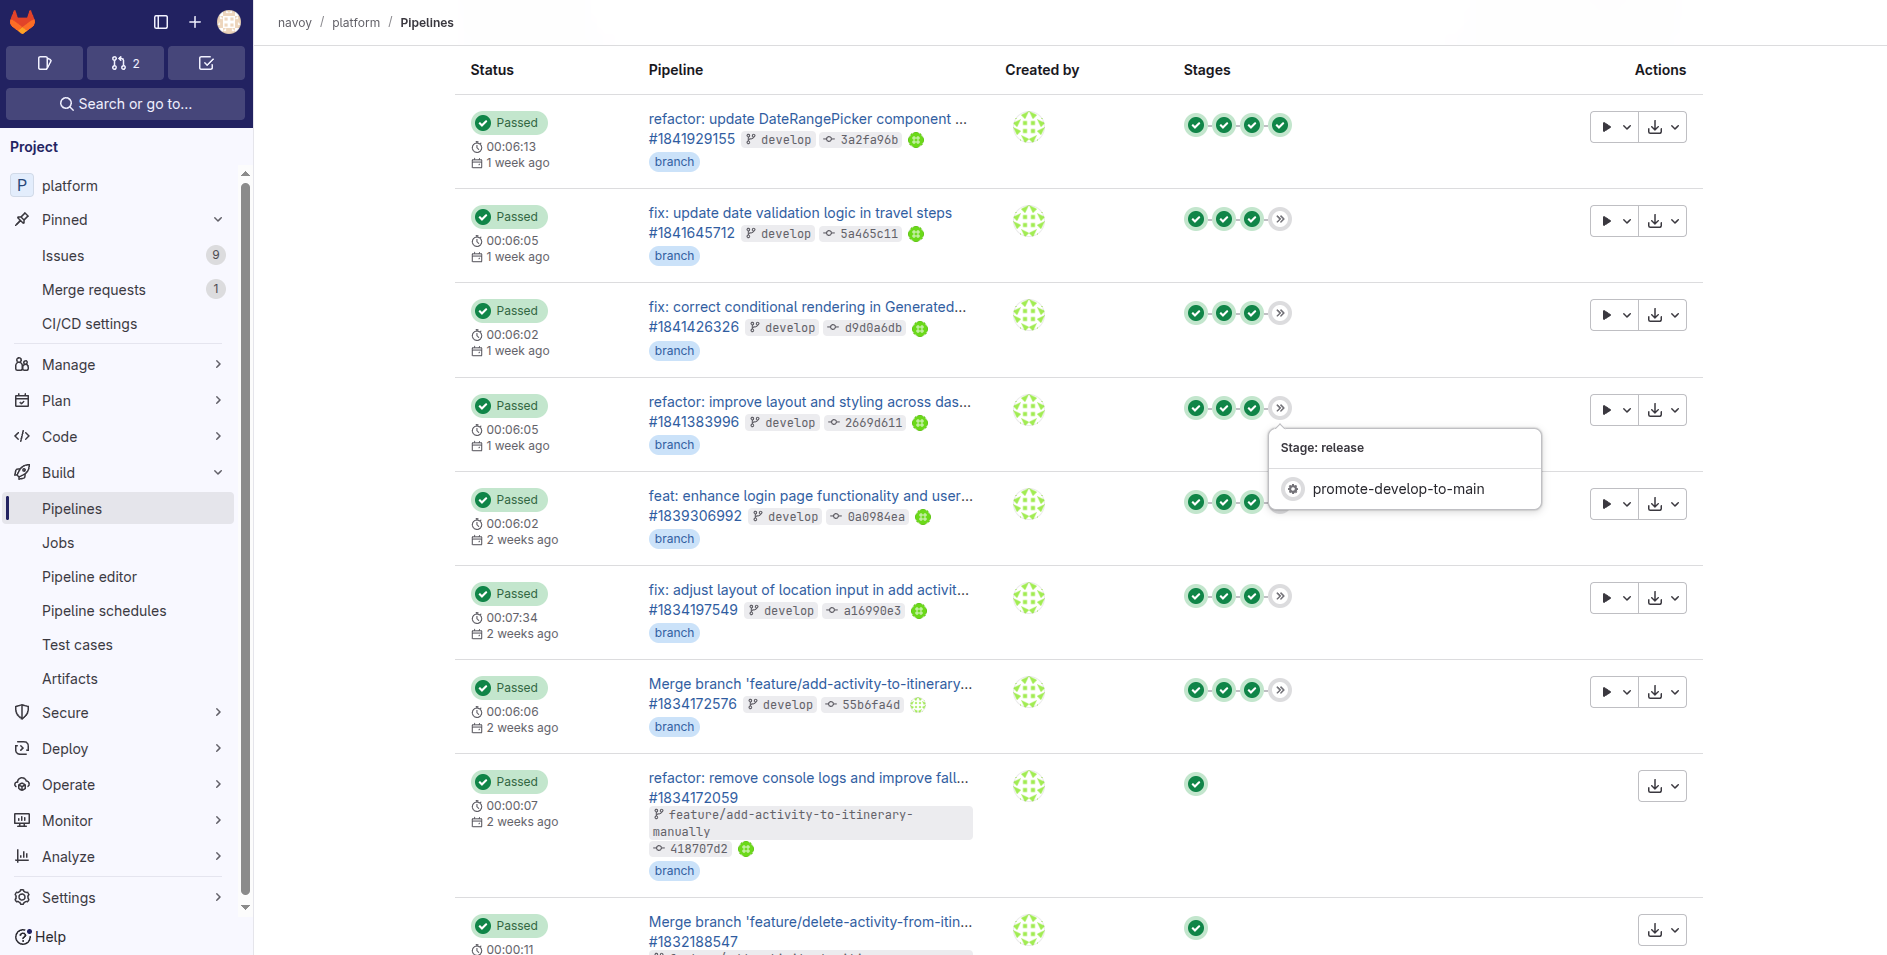
\includegraphics[width=\linewidth]{src/assets/images/pipeline-history-platform.png}}
    \caption{GitLab CI/CD Pipeline History - Platform Service Frontend Deployment}
    \label{fig:pipeline-history-platform}
\end{figure}

\subsection{Security Integration}
Comprehensive security measures are integrated throughout the development and deployment lifecycle.

\subsubsection*{\underline{Static Application Security Testing (SAST)}}
\begin{itemize}
    \item \textbf{Code Analysis:} Integrated SemGrep for static code analysis with custom rules for travel industry
    \item \textbf{Dependency Scanning:} Implemented Snyk for dependency vulnerability scanning
    \item \textbf{Secret Detection:} Added GitLeaks for preventing credential leaks in code repositories
    \item \textbf{Quality Gates:} Configured pipeline failure on high-severity security findings
\end{itemize}

\subsubsection*{\underline{Dynamic Application Security Testing (DAST)}}
\begin{itemize}
    \item \textbf{OWASP ZAP Integration:} Automated security testing against running applications
    \item \textbf{API Security Testing:} Implemented automated API security testing using custom scripts
    \item \textbf{Penetration Testing:} Scheduled weekly automated penetration tests on staging environment
    \item \textbf{Compliance Scanning:} Added compliance checks for GDPR and PCI DSS requirements
\end{itemize}

\subsection{Automated Testing Strategy}
Implemented comprehensive testing strategy covering unit, integration, and end-to-end testing.

\subsubsection*{\underline{Unit Testing Implementation}}
\begin{itemize}
    \item \textbf{Jest Configuration:} Achieved 85\% code coverage across all Node.js microservices
    \item \textbf{Pytest Setup:} Implemented comprehensive test suites for Python services with 80\% coverage
    \item \textbf{Mock Services:} Created mock services for external API dependencies
    \item \textbf{Test Data Management:} Implemented test database seeding and cleanup automation
\end{itemize}

\subsubsection*{\underline{End-to-End Testing with Playwright}}
Implemented comprehensive end-to-end testing using Playwright to simulate real user interactions with the travel platform. The tests cover the complete user journey from authentication through trip generation, including AI-powered itinerary creation workflows. Test scenarios include login processes, trip preference configuration, AI model interactions, and result validation with appropriate timeouts for AI processing.

\begin{figure}[H]
    \centering
    \makebox[\textwidth]{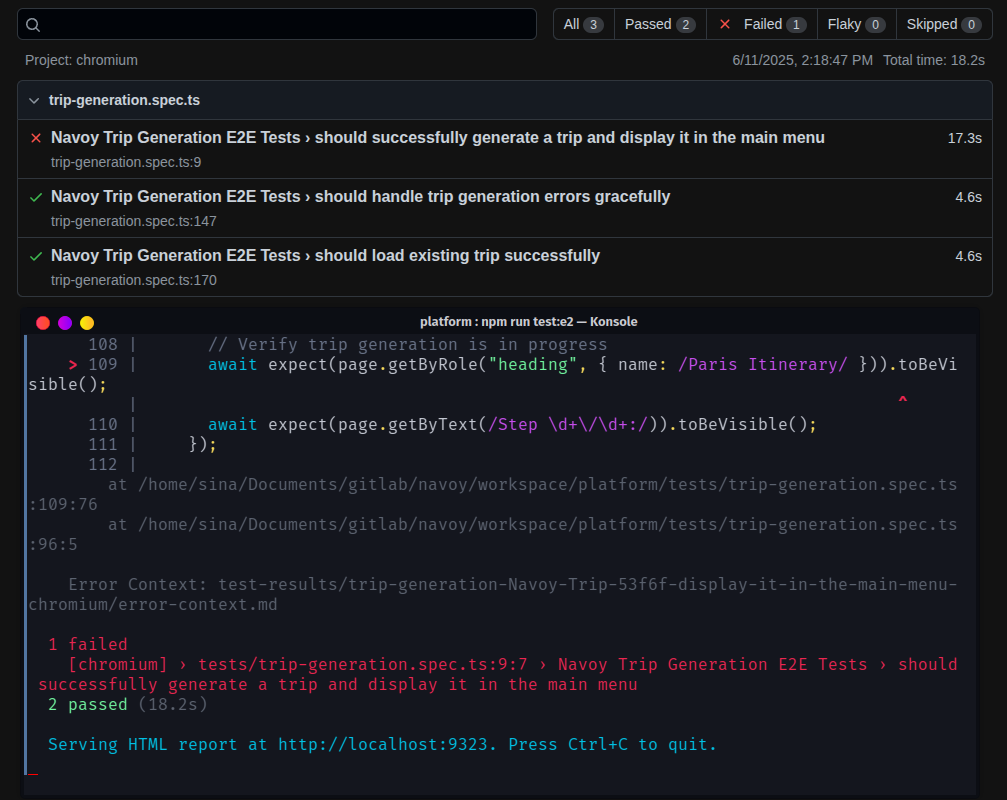
\includegraphics[width=\linewidth]{src/assets/images/playwright-testing.png}}
    \caption{Playwright End-to-End Testing Example}
    \label{fig:playwright-testing}
\end{figure}

\subsection{Deployment Automation}
Implemented blue-green deployment strategy with automated rollback capabilities and zero-downtime deployments.

\subsubsection*{\underline{Deployment Strategy}}
\begin{itemize}
    \item \textbf{Blue-Green Deployments:} Configured parallel environment deployments with traffic switching
    \item \textbf{Canary Releases:} Implemented gradual traffic shifting for production deployments
    \item \textbf{Health Checks:} Added comprehensive readiness and liveness probes for all services
    \item \textbf{Automated Rollback:} Configured automatic rollback on deployment failure or health check failures
\end{itemize}

% ----------------------- Monitoring and Observability ----------------------- %
\section{Monitoring and Observability Implementation}
Implemented comprehensive monitoring and observability stack to ensure platform reliability and performance optimization.

\subsection{Metrics Collection and Visualization}
Deployed Prometheus and Grafana for comprehensive metrics collection and visualization across all microservices.

\subsubsection*{\underline{Prometheus}}
Prometheus is an open-source monitoring and alerting toolkit designed for reliability and scalability. I use it to collect metrics from all microservices, infrastructure components, and external integrations. The system includes custom business metrics for tracking trip generation success rates, API usage patterns, and AI model performance. Prometheus provides real-time monitoring capabilities with configurable alert rules that notify the operations team of critical system events or performance degradations.

\subsubsection*{\underline{Grafana}}
Grafana is an open-source interactive visualization web application that provides rich dashboards for monitoring and analytics. I use it to visualize the metrics collected by Prometheus, creating comprehensive dashboards for system monitoring, application performance, and business KPIs. The implementation includes separate dashboard categories for infrastructure monitoring (CPU, memory, network, disk), service-specific metrics for each microservice, and business intelligence dashboards that track user engagement and platform usage patterns.

\subsection{Centralized Logging}
Implemented ELK Stack (Elasticsearch, Logstash, Kibana) for centralized log aggregation and analysis.

\subsubsection*{\underline{Elasticsearch}}
Elasticsearch serves as the central log storage and search engine for the entire platform. I configured it to handle large volumes of structured logs from all microservices, providing fast search capabilities and analytical processing. The implementation includes optimized indexing strategies, automated log rotation policies, and performance tuning to handle the high throughput requirements of the distributed system while maintaining query responsiveness.

\subsubsection*{\underline{Logstash}}
Logstash functions as the data processing pipeline that ingests, transforms, and forwards log data to Elasticsearch. I configured it to parse various log formats from different microservices, normalize timestamps, extract structured data from unstructured logs, and enrich log entries with additional context information. The pipeline includes filtering rules to handle different log levels and sources while maintaining data consistency across the entire logging infrastructure.

\subsubsection*{\underline{Kibana}}
Kibana provides the user interface for log analysis and visualization, allowing the operations team to search, filter, and analyze log data effectively. I created custom dashboards for different operational scenarios including error tracking, performance analysis, security monitoring, and business intelligence. The implementation includes saved searches for common troubleshooting scenarios and alerting configurations for critical log patterns.

\subsection{Distributed Tracing}
Deployed Jaeger for distributed tracing to monitor request flows across microservices.

\subsubsection*{\underline{Jaeger}}
Jaeger is an open-source distributed tracing system that helps monitor and troubleshoot transactions in complex distributed systems. I integrated Jaeger throughout the microservices architecture to provide end-to-end visibility of request flows, especially for complex operations like AI-powered trip generation that span multiple services. The implementation includes custom span instrumentation for AI model calls, external API interactions, and database operations, enabling detailed performance analysis and bottleneck identification.

% ----------------------- Technology Stack Summary ----------------------- %
\section{Technology Stack Summary}
This section summarizes all technologies implemented in the modernized Navoy AI travel platform.

\subsection{Programming Languages and Frameworks}

\subsubsection*{\underline{Node.js}}
Node.js 18 LTS serves as the primary runtime for the Vector Store Service and as the foundation for NestJS-based services. I chose Node.js for its excellent performance in handling concurrent API requests, its extensive ecosystem of middleware libraries, and strong TypeScript support. The implementation includes the Vector Store Service with gRPC server capabilities for high-performance vector similarity queries.

\subsubsection*{\underline{NestJS}}
NestJS serves as the primary framework for the User Service, Trip Generator Service, and Travel Data Sync Service. I chose NestJS for its enterprise-grade architecture, built-in TypeScript support, powerful dependency injection system, and comprehensive decorator-based approach. The framework provides robust support for microservices architecture, database integration, and API development with automatic OpenAPI documentation generation.

\subsubsection*{\underline{Envoy Proxy}}
Envoy Proxy functions as the service mesh and API gateway, replacing traditional Express.js-based gateway implementations. I selected Envoy for its advanced traffic management capabilities, built-in observability features, dynamic configuration support, and proven performance in high-throughput scenarios. The implementation includes sophisticated routing, rate limiting, authentication, and load balancing features.

\subsubsection*{\underline{TypeScript}}
TypeScript enhances code quality and developer productivity across all Node.js services and frontend development. It provides compile-time type checking, better IDE support, and improved maintainability for large codebases. The implementation includes strict TypeScript configurations and custom type definitions for API contracts.

\subsubsection*{\underline{gRPC}}
gRPC serves as the high-performance communication protocol for the Vector Store Service, providing efficient binary serialization and bi-directional streaming capabilities. I chose gRPC for its superior performance characteristics compared to REST APIs, especially for high-frequency vector similarity queries. The implementation includes Protocol Buffer definitions for type-safe communication and automatic client generation for multiple languages.

\subsubsection*{\underline{TypeScript}}
TypeScript enhances code quality and developer productivity across all Node.js and NestJS services. It provides compile-time type checking, better IDE support, and improved maintainability for large codebases. The implementation includes strict TypeScript configurations, custom type definitions for API contracts, and comprehensive decorator-based architecture with NestJS.

\subsection{Databases and Storage Solutions}

\subsubsection*{\underline{PostgreSQL}}
PostgreSQL 15 serves as the primary relational database for the User Service and Billing Service, providing ACID compliance for transactional data. I chose PostgreSQL for its robust feature set including row-level security for multi-tenancy, advanced indexing capabilities, and excellent support for JSON data types. The implementation includes optimized schemas, connection pooling, and automated backup procedures.

\subsubsection*{\underline{MongoDB}}
MongoDB 6.0 handles document storage for the Trip Generator and Data Sync services where flexible schema design is crucial. Its document-oriented approach perfectly suits the varying structures of travel data from different providers and AI-generated content. The implementation includes sharding strategies, replica sets for high availability, and optimized indexing for travel data queries.

\subsubsection*{\underline{Redis}}
Redis 7.0 provides high-performance caching and session management across the platform. I use it for gateway response caching, rate limiting counters, session storage, and as a message broker for real-time features. The implementation includes clustering for high availability and optimized memory usage patterns.

\subsubsection*{\underline{ChromaDB}}
ChromaDB serves as the specialized vector database for the Vector Store Service, enabling semantic search capabilities and AI embedding storage. Its purpose-built design for vector operations makes it ideal for AI-powered travel recommendations and similarity searches. The implementation includes optimized vector indexing and query performance tuning.

\subsubsection*{\underline{S3 Compatible Storage}}
S3-compatible object storage handles static assets for the CMS Service and provides reliable backup storage. The implementation includes lifecycle policies for cost optimization, versioning for data protection, and CDN integration for global content delivery.

\subsubsection*{\underline{Elasticsearch}}
Elasticsearch provides powerful search and analytics capabilities for centralized logging and business intelligence. Its distributed architecture handles large volumes of log data while maintaining fast query performance. The implementation includes optimized mapping strategies and automated index management.

\subsection{DevSecOps and Infrastructure Technologies}

\subsubsection*{\underline{Kubernetes}}
Kubernetes 1.28 orchestrates the entire containerized infrastructure using Amazon EKS managed Kubernetes service. I chose EKS for its robust container orchestration capabilities, automatic scaling, service discovery, rolling deployment features, and integrated AWS service support. The implementation includes managed node groups, network policies for security, and comprehensive monitoring integration with AWS CloudWatch.

\subsubsection*{\underline{Docker}}
Docker provides containerization for all microservices with optimized multi-stage builds and comprehensive security scanning. The implementation emphasizes minimal attack surfaces through Alpine Linux base images, non-root user configurations, and automated vulnerability assessment in the CI/CD pipeline.

\subsubsection*{\underline{Helm}}
Helm 3.12 manages Kubernetes deployments through templated charts, ensuring consistent configuration across environments. The implementation includes parameterized deployments, dependency management, and automated rollback capabilities for reliable application lifecycle management.

\subsubsection*{\underline{Terraform}}
Terraform 1.5 implements Infrastructure as Code for AWS resource provisioning and management. The implementation includes modular configurations, state management, and automated drift detection to ensure infrastructure consistency and reproducibility across environments.

\subsubsection*{\underline{GitLab CI/CD}}
GitLab CI/CD provides comprehensive DevSecOps pipeline automation with integrated security scanning and deployment orchestration. The implementation includes parallel execution stages, comprehensive artifact management, and automated promotion between environments while maintaining security gates throughout the pipeline.

\subsection{AI and Integration Technologies}

\subsubsection*{\underline{LiteLLM}}
LiteLLM serves as a unified proxy for accessing multiple AI language models, providing consistent API interfaces and intelligent routing capabilities. I use it to abstract away the complexities of different AI providers while implementing cost optimization through smart model selection based on request complexity and caching strategies.

\subsubsection*{\underline{OpenAI GPT-4}}
OpenAI GPT-4 functions as the primary AI model for creative trip generation and complex travel planning scenarios. Its advanced reasoning capabilities and extensive training data make it ideal for generating detailed, personalized travel itineraries with cultural insights and local recommendations.

\subsubsection*{\underline{Anthropic Claude}}
Anthropic Claude provides secondary AI capabilities, particularly for detailed travel advice and safety considerations. Its focus on helpful, harmless, and honest responses makes it valuable for travel safety recommendations and detailed destination information.

\subsubsection*{\underline{AWS Bedrock}}
AWS Bedrock provides managed access to foundation models from multiple AI providers, including Anthropic Claude models, for advanced AI capabilities within the AWS production environment. The service enables seamless integration with Claude models for trip evaluation, optimization, and enhanced recommendation generation without the complexity of managing model infrastructure. Through Bedrock, the platform can access Claude's advanced reasoning capabilities for travel safety assessments, cultural sensitivity recommendations, and complex multi-destination trip planning scenarios while maintaining enterprise-grade security and compliance within the AWS ecosystem.

\begin{figure}[H]
    \centering
    \makebox[\textwidth]{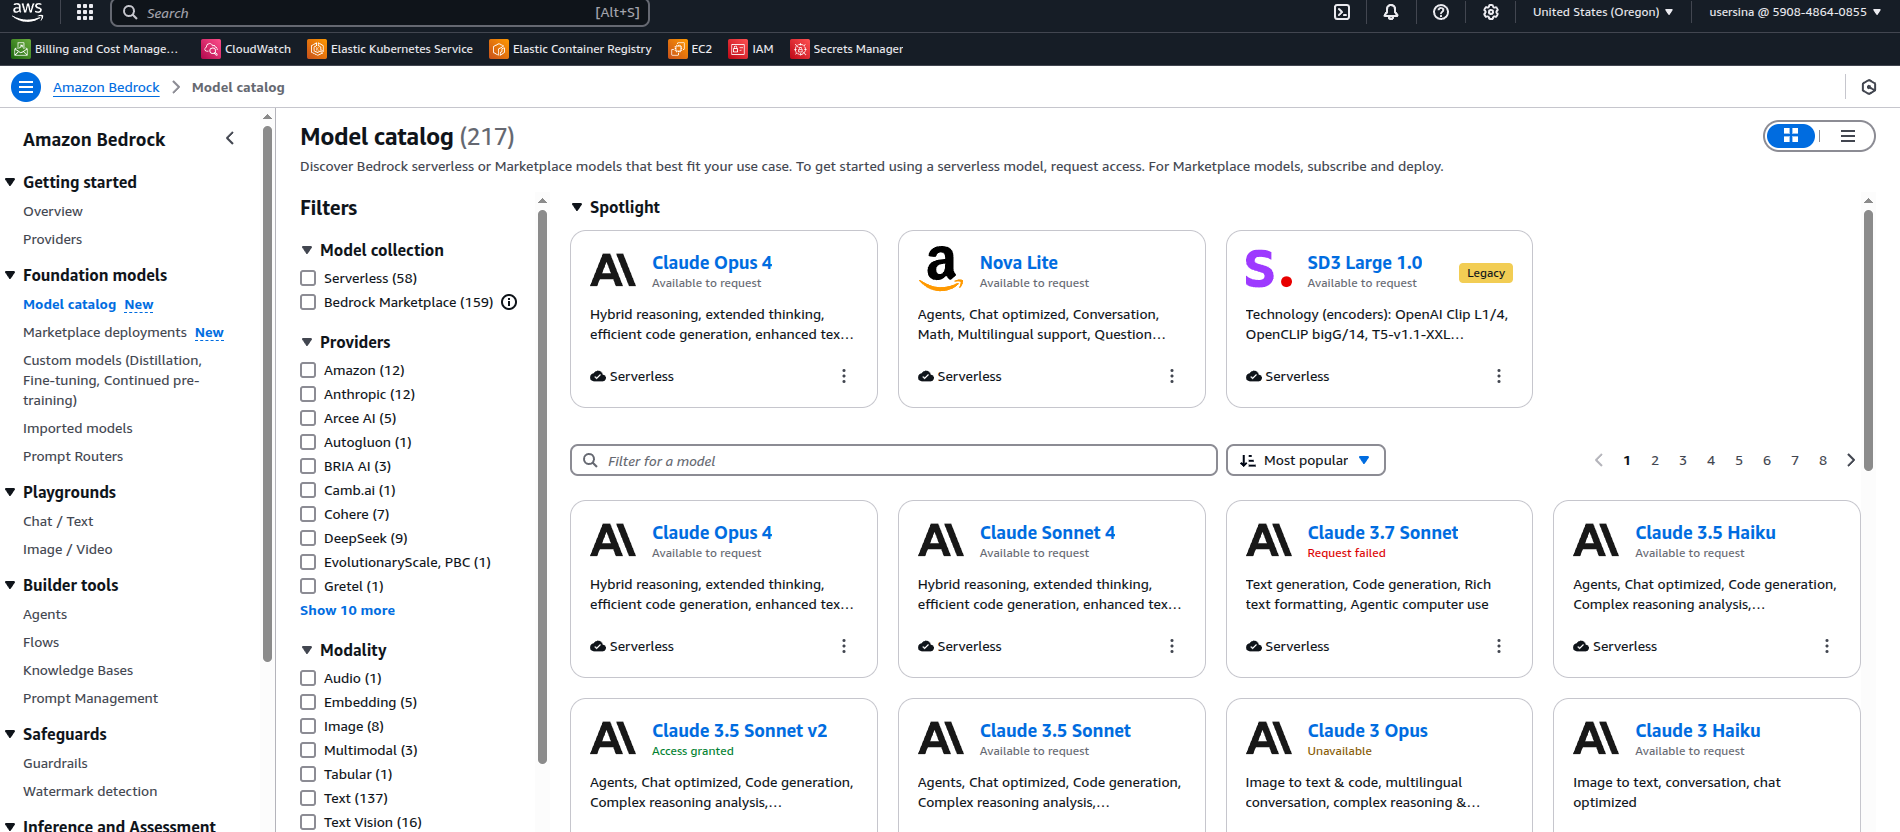
\includegraphics[width=\linewidth]{src/assets/images/aws-bedrock-model-catalog.png}}
    \caption{AWS Bedrock Model Catalog - Foundation Model Selection Interface}
    \label{fig:aws-bedrock-model-catalog}
\end{figure}

\subsubsection*{\underline{Amazon SQS/SNS}}
Amazon SQS and SNS serve as the message queuing and notification services for asynchronous processing and service decoupling. The implementation includes durable queues through SQS, message fan-out via SNS, and dead letter queues for handling failed processing scenarios while maintaining data integrity across distributed operations. These services integrate seamlessly with AWS Lambda for event-driven serverless processing.

\subsubsection*{\underline{AWS Lambda}}
AWS Lambda provides serverless compute functionality for background job processing, particularly for AI model calls and data synchronization tasks. The implementation includes automatic scaling based on demand, cost-effective pay-per-execution pricing, and seamless integration with other AWS services. Lambda functions handle asynchronous trip generation processing, scheduled data synchronization, and event-driven workflows while eliminating infrastructure management overhead.

\subsubsection*{\underline{Stripe API}}
Stripe API handles payment processing for both subscription-based and pay-per-use billing models. The integration includes webhook handling for real-time payment status updates, subscription management, and compliance with PCI DSS requirements.

\subsubsection*{\underline{Viator API}}
Viator API integration provides comprehensive tours and activities data through a dedicated adapter service. The implementation includes rate limiting, data transformation, and caching strategies to optimize performance while staying within API quotas.

\subsubsection*{\underline{Amadeus API}}
Amadeus API synchronizes flight and hotel data to provide comprehensive travel information. The integration includes intelligent caching, delta synchronization, and fallback mechanisms to ensure data availability even during API outages.

% ----------------------- Technical Challenges and Solutions ----------------------- %
\section{Technical Challenges and Solutions}
During the implementation of Navoy's modernized AI travel platform, I encountered several significant technical challenges that required innovative solutions.

\subsection{Microservices Data Consistency}
\textbf{Challenge:} Maintaining data consistency across multiple microservices while ensuring service autonomy and avoiding distributed transactions.

\textbf{Solution:} Implemented the Saga pattern with event-driven architecture using Amazon SNS and SQS. Each service publishes domain events to SNS topics when data changes occur, and other services subscribe via SQS queues to relevant events to maintain their local data consistency. Added compensation mechanisms using AWS Lambda functions for handling failures in distributed operations.

\subsection{AI Model Cost Optimization}
\textbf{Challenge:} Managing costs associated with AI model usage while maintaining response quality and availability.

\textbf{Solution:} Implemented intelligent model routing through LiteLLM based on request complexity. Simple requests use GPT-3.5-turbo while complex multi-destination trips use GPT-4. Added response caching for similar requests and implemented request preprocessing to optimize token usage.

\subsection{External API Rate Limiting}
\textbf{Challenge:} Managing rate limits from external travel APIs (Viator, Amadeus) while ensuring fresh data availability.

\textbf{Solution:} Implemented an intelligent rate limiting system with exponential backoff and circuit breaker patterns. Added data freshness scoring to prioritize synchronization of stale data and implemented API key rotation to increase throughput limits.

\subsection{Kubernetes Persistent Storage}
\textbf{Challenge:} Managing persistent storage for stateful services like databases while maintaining scalability and data durability.

\textbf{Solution:} Implemented StatefulSets for database deployments with persistent volume claims. Added automated backup and restore procedures using Velero. Configured storage classes with appropriate retention policies and implemented data encryption at rest.

\subsection{Distributed Debugging and Tracing}
\textbf{Challenge:} Debugging issues across multiple microservices and understanding request flows in a distributed system.

\textbf{Solution:} Implemented comprehensive distributed tracing using Jaeger with OpenTelemetry instrumentation. Added correlation IDs to all requests and enhanced logging with structured JSON format. Created custom dashboards in Grafana for visualizing service dependencies and performance metrics.

\subsection{Security Scanning Integration}
\textbf{Challenge:} Integrating comprehensive security scanning without significantly impacting CI/CD pipeline performance.

\textbf{Solution:} Implemented parallel security scanning stages in GitLab CI/CD pipeline. Added container image caching to reduce scan times and configured incremental scanning for code changes. Implemented security gates that fail builds only on high-severity vulnerabilities while logging medium and low-severity issues for later review.

\subsection{Multi-Environment Configuration Management}
\textbf{Challenge:} Managing configuration differences between development, staging, and production environments while maintaining security.

\textbf{Solution:} Implemented GitOps approach with separate Helm values files for each environment. Used sealed-secrets for Kubernetes secret management and AWS Secrets Manager for external service credentials. Added environment-specific validation and testing procedures.

\setcounter{secnumdepth}{0} % Set the section counter to 0 so next section is not counted in toc
% ----------------------- Conclusion ----------------------- %
\section{Conclusion}
This chapter detailed the successful implementation of Navoy's modernized AI travel platform, transforming from a monolithic architecture to a scalable microservices ecosystem using comprehensive DevSecOps practices.

Key achievements include AI-powered trip generation, robust monitoring with Prometheus and Grafana, automated CI/CD pipelines with security scanning, and infrastructure deployment using Terraform and Kubernetes. The platform now provides a solid foundation that can scale to meet growing demands while maintaining security and reliability standards.
